\documentclass{article}
\usepackage[utf8]{inputenc}

\title{Relay Node Placement Problem}
\author{Zackary Crosley\thanks{Names are listed in alphabetical order.}, Maxfield Lehman$^*$, and Zahra Zahedi$^*$}
\date{March 2019}

\usepackage{natbib}
\usepackage{graphicx}
\usepackage{amssymb}
\usepackage{amsmath}
\usepackage{mathtools}
\usepackage{amsthm}
\usepackage{listings}

\begin{document}

\maketitle

\section{Introduction}
In this project we study the problem of relay node deployment, where a number of sensors have been placed in a deployment area and the goal is to place the relay nodes while optimizing for various connectedness properties. In this problem, we have limitations on the placement of relay nodes due to the cost associated with them. As a result, we may not have sufficient relay nodes to make the entire network connected. This is why we instead optimize for a "high" level of connection where the definition of "highly connected" varies based on which connectedness property we deem most important. Our reference paper \cite{relay-node} (henceforth referred to as 'the paper') used a notion of connectedness for a partially disconnected graph and then introduced two explicit metrics to measure this connectedness. These metrics are as follows:
\begin{itemize}
    \item The number of components of a graph in which a lower number of components indicates a higher degree of connectedness of a graph.
    \item The size of the largest component of the graph where the larger size indicates a higher degree of connectedness.
\end{itemize}
Note that a component refers to a subset $V$ of the graph's vertices which are connected. In our problem, this corresponds to a subgraph of the desired measurement areas induced by V.

\section{Problem Formulation}
As discussed in the Introduction, we have two metrics for connectedness. In both of them, we have 1. A set $P=\{p_1, \hdots, p_n\}$ which is the location of sensor nodes in Euclidean plane, 2. A communication range $R$ related to the sensors and relay nodes, and 3. A budget $B$  on the number of relay nodes. We would have a graph $G=(V,E)$ where $v_i\in V$ is a node from each point $p_i\in P$, and $v_i$, $v_j$ are two nodes with edge $e_{ij}\in E$, if the distance between $p_i$ and $p_j$ are less than $R$. This graph $G(V, E)$ may be disconnected with some number of connected components. Thus, we can have an augmented graph $G^\prime=(V^\prime, E^\prime)$ connected, which includes sensors and relay nodes, where $Q=\{q_1, \hdots, q_{|B|}\}$ are the location of $B$ deployed relay nodes. For our goal, we must obtain a graph $G^\prime=(V^\prime, E^\prime)$ with maximal connectedness as measured by the number of components of $G^\prime=(V^\prime, E^\prime)$ or by the size of the largest component of $G^\prime=(V^\prime, E^\prime)$.

\section{Problem Solutions}
\subsubsection*{First Solution}For minimizing the number of connected components of $G^\prime$, the paper \cite{relay-node} has introduced the \textbf{\textit{Budget Constrained Relay node Placement with Minimum Number of Connected Component (BCRP-MNCC)}} algorithm. Given the location of $n$ sensor nodes $P=\{p_1, \hdots, p_n\}$, and communication range $R$, a constant $C$ and budget $B_1$, we can find a set $Q=\{q_1, \hdots, q_{|B|}\}$ as the location of deployed relay-node so that the number of components in the graph $G^\prime=(V^\prime, E^\prime)$ is at most $C$. \\
The following algorithm is the heuristic solution to this problem offered by \cite{relay-node}.
\begin{figure}[h]
\centering
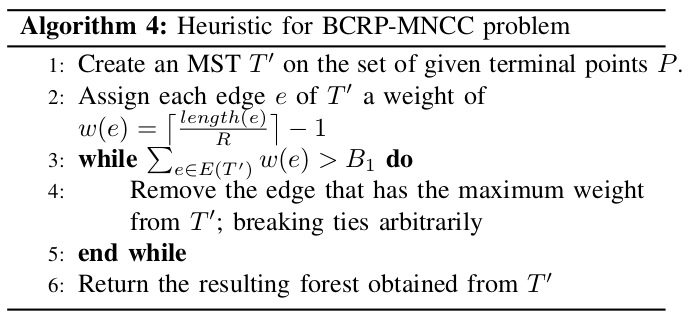
\includegraphics[width=0.9\textwidth]{Alg4.png}
\label{alg4}
\caption{Algorithm 4 from Mazumder et. al.}
\end{figure}\\

As can be seen in Figure 1, calculating the location of relay-nodes that minimizes the number of components utilizes iterative reduction of a minimum spanning tree (MST). A minimum spanning tree returns the shortest possible way of connecting all the vertices of the graph. In an ideal case, this minimum spanning tree would provide us a solution to how to place our relay nodes with a single connected network. However, this is not possible in all cases. In conditions with limited resources connecting all components may not be feasible. The algorithm introduces the concept of a budget as an upper limit, where the cost being minimized is a ratio of the euclidean distance and the communication range for a relay node. Since we are operating on a minimum spanning tree at first and on minimally-connected components in subsequent iterations, removing a single edge results in the creation of an additional component. We remove the largest cost edges in the tree necessary to fall under our budget, resulting in the minimum number of edges being removed. In this way, we minimize the number of connected components.\\

\subsubsection*{Second Solution}
To maximize the size of the largest connected component of $G^\prime$, we have \textbf{\textit{Budget Constrained Relay node Placement with Maximum size of Largest Connected Component (BCRP-MLCC)}} where given the location of $n$ sensor nodes $P=\{p_1, \hdots, p_n\}$, and communication range $R$, a constant $C$ and budget $B_2$, we can find a set $Q=\{q_1, \hdots, q_{|B|}\}$ as the location of deployed relay-node so that the size of the largest connected component in the graph $G^\prime=(V^\prime, E^\prime)$ is at least $C$. The algorithm is give as follows.
\begin{figure}[h]
\centering
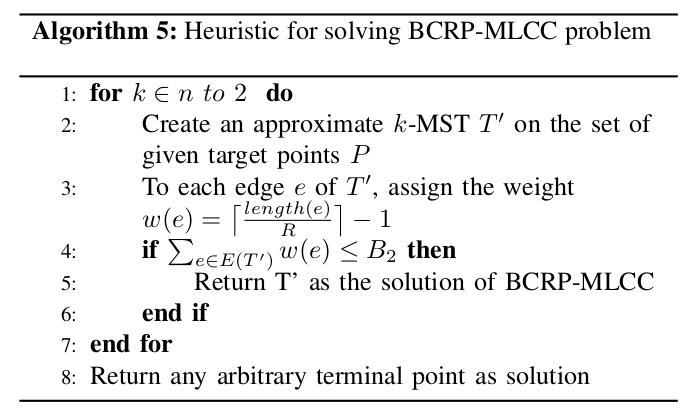
\includegraphics[width=0.9\textwidth]{Alg5.png}
\label{alg5}
\caption{Algorithm 5 from Mazumder et. al.}
\end{figure}\\

To determine the locations of relay-nodes that maximizes the size of the largest connected component, we find the largest approximate minimum spanning tree that comes under budget. To do this we implement a k-minimum spanning tree (k-MST) approximation. The k-MST problem is to find a minimum spanning tree of k vertices and is NP-Hard, but many approximations with varying bounds exist. A k-minimum spanning tree with $k = \left|V\right|$ would be equivalent to the MST algorithm. In this implementation we iteratively decrement the value of k from the number of vertices in the graph n to a minimum of two. With each k, we calculate the k-MST. If the resulting MST is under budget, that tree is returned as the largest possible component under budget. Else, we continue with a decremented value for k.

\section{Implementation of The Algorithms}
We chose to implement this project in Clojure for several reasons, but particularly the spiritual enlightenment attained from working with graphs and trees from within a language whose source is itself directly manipulated as a tree. Tying into this, Clojure has a well-defined protocol for graph operations called Loom, enabling us to choose any of the various Loom implementations based on their ergonomics. Since we knew we would be implementing algorithms from the graph primitives provided by Loom and any implementation thereof, these ergonomics were of particular importance. For instance, implementing both algorithms described above requires the calculation of minimum spanning trees. In the first case, Algorithm 4 from the paper, this is a standard fully spanning tree, while the next algorithm requires k-minimal spanning trees. The main benefits of Clojure for our implementation in this case are two-fold: a base protocol that would allow us to swap implementations later if we ran into teething issues with our initial choice of implementation and maximum code flexibility which allows us to wrap any unwieldy aspects of library APIs with minimal effort.

An important part of our implementation has been our use of a disjoint-set library in the process of computing minimum spanning trees, which leans heavily on the disjoint set data structure. We weren't sure if this was something we were expected to implement ourselves for this algorithm, so we implemented a set of lightweight wrapper functions to allow swapping this library out for an implementation of our own if that turns out to be required.

These well-designed abstractions allow us to implement the required algorithms with minimal cognitive overhead and with our code neatly mapping onto the psuedocode given in the paper. For example, compare the following code snippet to Figure 1:

\begin{lstlisting}{clojure}
(defn algorithm4
  [graph comm-range budget]
  (let [mst      (minimum-spanning-tree graph)
        weighted (atom (weight-tree mst comm-range))]
    (while (> (total-edge-weight @weighted)
              budget)
      (swap! weighted
             remove-edge
             (max-edge-by @weighted :weight)))
    @weighted))
\end{lstlisting}

The main roadblock for our implementation going forward is selecting an appropriate k-minimum-spanning-tree algorithm that applies straightforwardly to our domain while balancing approximation correctness against implementation complexity. We have found a variety of relevant algorithms and are evaluating them. Currently, we do not have a clear best choice but hope to resolve this quickly.

\section{Result}
We have successfully implemented the first of the two algorithms from the paper, which is the budget constrained relay node placement with minimum number of connected components (BCRP-MNCC). This algorithm finds the optimal placement of nodes to minimize the number of separate networks of relay nodes. To accomplish this, we first used a graph library in Clojure and implemented a generic minimum spanning tree (MST) function. We then implemented the fourth algorithm from the paper using this and other utility functions and evaluated its results using randomly generated graphs as input. Our manual testing shows correct output, suggesting a completed implementation.

The second algorithm to implement, algorithm 5 from the paper, is the budget constrained relay node placement with maximum size of largest connected component (BCRP-MLCC). This algorithm finds the optimal node placement for sensors given a budget while maximizing the number of nodes in a single large component. This problem is still being researched before implementation. The algorithm is built off of a k-node minimum spanning tree, the calculation of which is an NP-Hard problem. As such this algorithm is an approximation, and many different implementations exist. We are still exploring the different implementations to determine which is best for our use case. One question we are trying to answer in order to make this determination is what type of k-MST is best for this problem. Some k-MST implementations require an initial root node, which may or may not be a good decision for this algorithm. Once this determination is made, we will implement the k-MST on top of our chosen graph structure, after which the completion of this algorithm is straight forward.

\section{Conclusion}

This project discusses and implements two algorithms designed to make placement decisions for sensor relay nodes in a limited budget environment. We implement algorithms that perform this placement while using either number of components or largest component as a placement metric. We have completed the first of the two algorithms and validated its accuracy. We are evaluating which k-MST algorithm to implement for the second algorithm, after which the remaining portion of BCRP-MLCC should be trivial to implement. We are well on track for the project to be completed and written up on time.

%\begin{figure}[h!]
%\centering
%\includegraphics[scale=1.7]{universe}
%\caption{The Universe}
%\label{fig:universe}
%\end{figure}



\bibliographystyle{plain}
\bibliography{references}
\end{document}
